\section{Exercises}
\label{section:representationsExercises}
\graphicspath{ {./chapter02/FigHw} }

\begin{enumerate}
    \item \textbf{(2 pts. each)} Given: $F(A,B,C,D) = (AB' + (C+(AD)')(BD))'$

        \begin{enumerate}
            \item Determine the truth table for $F(A,B,C,D)$

                \begin{onlysolution}  \textbf{Solution} \itshape

                    Let T1 = AB'\\
                    T2 = (AD)'\\
                    T3 = C+(AD)'\\
                    T4 = BD\\
                    T5 = T3 $\cdot$ T4\\

                    \begin{tabular}{l|l|l|l|l|l|l|l|l|l|l}
                        A &  B &  C &  D & AB' & (AD)' & C+(AD)' & BD & T3*T4 & T1+T5  &  F  \\ \hline \rowcolor{gray!15}
                        0 &  0 &  0 &  0 &  0 &  1     &  1      &  0 &  0    &  0     &  1  \\ \hline
                        0 &  0 &  0 &  1 &  0 &  1     &  1      &  0 &  0    &  0     &  1  \\ \hline \rowcolor{gray!15}
                        0 &  0 &  1 &  0 &  0 &  1     &  1      &  0 &  0    &  0     &  1  \\ \hline
                        0 &  0 &  1 &  1 &  0 &  1     &  1      &  0 &  0    &  0     &  1  \\ \hline \rowcolor{gray!15}
                        0 &  1 &  0 &  0 &  0 &  1     &  1      &  0 &  0    &  0     &  1  \\ \hline
                        0 &  1 &  0 &  1 &  0 &  1     &  1      &  1 &  1    &  1     &  0  \\ \hline \rowcolor{gray!15}
                        0 &  1 &  1 &  0 &  0 &  1     &  1      &  0 &  0    &  0     &  1  \\ \hline
                        0 &  1 &  1 &  1 &  0 &  1     &  1      &  1 &  1    &  1     &  0  \\ \hline \rowcolor{gray!15}
                        1 &  0 &  0 &  0 &  1 &  1     &  1      &  0 &  0    &  1     &  0  \\ \hline
                        1 &  0 &  0 &  1 &  1 &  0     &  0      &  0 &  0    &  1     &  0  \\ \hline \rowcolor{gray!15}
                        1 &  0 &  1 &  0 &  1 &  1     &  1      &  0 &  0    &  1     &  0  \\ \hline
                        1 &  0 &  1 &  1 &  1 &  0     &  1      &  0 &  0    &  1     &  0  \\ \hline \rowcolor{gray!15}
                        1 &  1 &  0 &  0 &  0 &  1     &  1      &  0 &  0    &  0     &  1  \\ \hline
                        1 &  1 &  0 &  1 &  0 &  0     &  0      &  1 &  0    &  0     &  1  \\ \hline \rowcolor{gray!15}
                        1 &  1 &  1 &  0 &  0 &  1     &  1      &  0 &  0    &  0     &  1  \\ \hline
                        1 &  1 &  1 &  1 &  0 &  0     &  1      &  1 &  1    &  1     &  0  \\
                    \end{tabular}
                \end{onlysolution}

            \item Draw a schematic of the logic circuit which realizes $F$ as
                shown, i.e. do not use Boolean Algebra on $F$.

                \begin{onlysolution}  \textbf{Solution} \itshape
                    \begin{figure}[ht]
                        
\includegraphics{Sol2-1}
                    \end{figure}
                \end{onlysolution}
        \end{enumerate}

    \item \textbf{(2 pts. each)} For the circuit in Figure~\ref{fig:representationsHwCir2Bool}
        \begin{enumerate}
            \item Write a Boolean expression for the function.

                \begin{onlysolution}  \textbf{Solution} \itshape
                    F(A,B,C,D) = (AB+C)D'+ABD'
                \end{onlysolution}
                \filbreak
            \item Draw the truth table for the function.\penalty0

                \begin{onlysolution}  \textbf{Solution} \itshape

                    \begin{tabular}{l|l|l|l|l|l|l|l}
                        A &  B &  C &  D & AB+C  & (AB+C)D' & ABD'  &  F    \\ \hline \rowcolor{gray!15}
                        0 &  0 &  0 &  0 &  0 &  0 &  0 &  0                \\ \hline
                        0 &  0 &  0 &  1 &  0 &  0 &  0 &  0                \\ \hline \rowcolor{gray!15}
                        0 &  0 &  1 &  0 &  1 &  0 &  0 &  1                \\ \hline
                        0 &  0 &  1 &  1 &  1 &  1 &  0 &  0                \\ \hline \rowcolor{gray!15}
                        0 &  1 &  0 &  0 &  0 &  0 &  0 &  0                \\ \hline
                        0 &  1 &  0 &  1 &  0 &  0 &  0 &  0                \\ \hline \rowcolor{gray!15}
                        0 &  1 &  1 &  0 &  1 &  0 &  0 &  1                \\ \hline
                        0 &  1 &  1 &  1 &  1 &  1 &  0 &  0                \\ \hline \rowcolor{gray!15}
                        1 &  0 &  0 &  0 &  0 &  0 &  0 &  0                \\ \hline
                        1 &  0 &  0 &  1 &  0 &  0 &  0 &  0                \\ \hline \rowcolor{gray!15}
                        1 &  0 &  1 &  0 &  1 &  0 &  0 &  1                \\ \hline
                        1 &  0 &  1 &  1 &  1 &  1 &  0 &  0                \\ \hline \rowcolor{gray!15}
                        1 &  1 &  0 &  0 &  1 &  0 &  1 &  1                \\ \hline
                        1 &  1 &  0 &  1 &  1 &  1 &  0 &  0                \\ \hline \rowcolor{gray!15}
                        1 &  1 &  1 &  0 &  1 &  0 &  1 &  1                \\ \hline
                        1 &  1 &  1 &  1 &  1 &  0 &  0 &  0                \\
                    \end{tabular}
                \end{onlysolution}
        \end{enumerate}
        \begin{figure}[ht]
            
\includegraphics{Prob2-3}
            \caption{The circuit for Problems 2 and 3.}
            \label{fig:representationsHwCir2Bool}
        \end{figure}

    \item \textbf{ (2 pts. each)} For the functions F,G,H,I defined by the
        truth table shown below:
        \begin{enumerate}
            \item Determine the canonical SOP and POS realization for $F,G,H,I$.

                {
                    \begin{onlysolution}\textbf{Solution}\vspace{-1em}

                        \hspace*{-47pt}\vbox{
                            \begin{align*} % The width of H spills into the right margin. To fix it, we move
                                % the entire block over by the width it overflowed the hbox by. However, an
                                % align environment is a floating environment, so we need to use a vbox to move it over.
                                F(A,B,C) &= (A+B+C)(A+B'+C')(A'+B+C')(A'+B'+C)  \\
                                &= \phantom{(}A'B'C + A'BC' + AB'C' + ABC \\[0.2ex] % The phantom is used to
                                    % align the first term between SOP and POS. the 0.2ex is used to add a
                                    % little extra space between each set of answers
                                    G(A,B,C) &= (A'+B+C)(A'+B'+C') \\
                                    &= \phantom{(}A'B'C' + A'B'C + A'BC' + A'BC + AB'C + ABC'  \\[0.2ex]
                                        H(A,B,C) &= (A+B'+C)(A+B'+C')(A'+B+C)(A'+B+C')(A'+B'+C') \\
                                        &= \phantom{(}A'B'C' + A'B'C + ABC' \\[0.2ex]
                                            I(A,B,C) &= (A+B+C)(A+B'+C)(A'+B+C)(A'+B'+C) \\
                                            &= \phantom{(}A'B'C + A'BC + AB'C + ABC
                                        \end{align*}}
                                \end{onlysolution}}

                            \item Draw the circuit diagram for the canonical SOP and POS
                                realization.
                                \begin{onlysolution}
                                    \begin{figure}[htp]
                                        \textbf{Solution}\\
                                        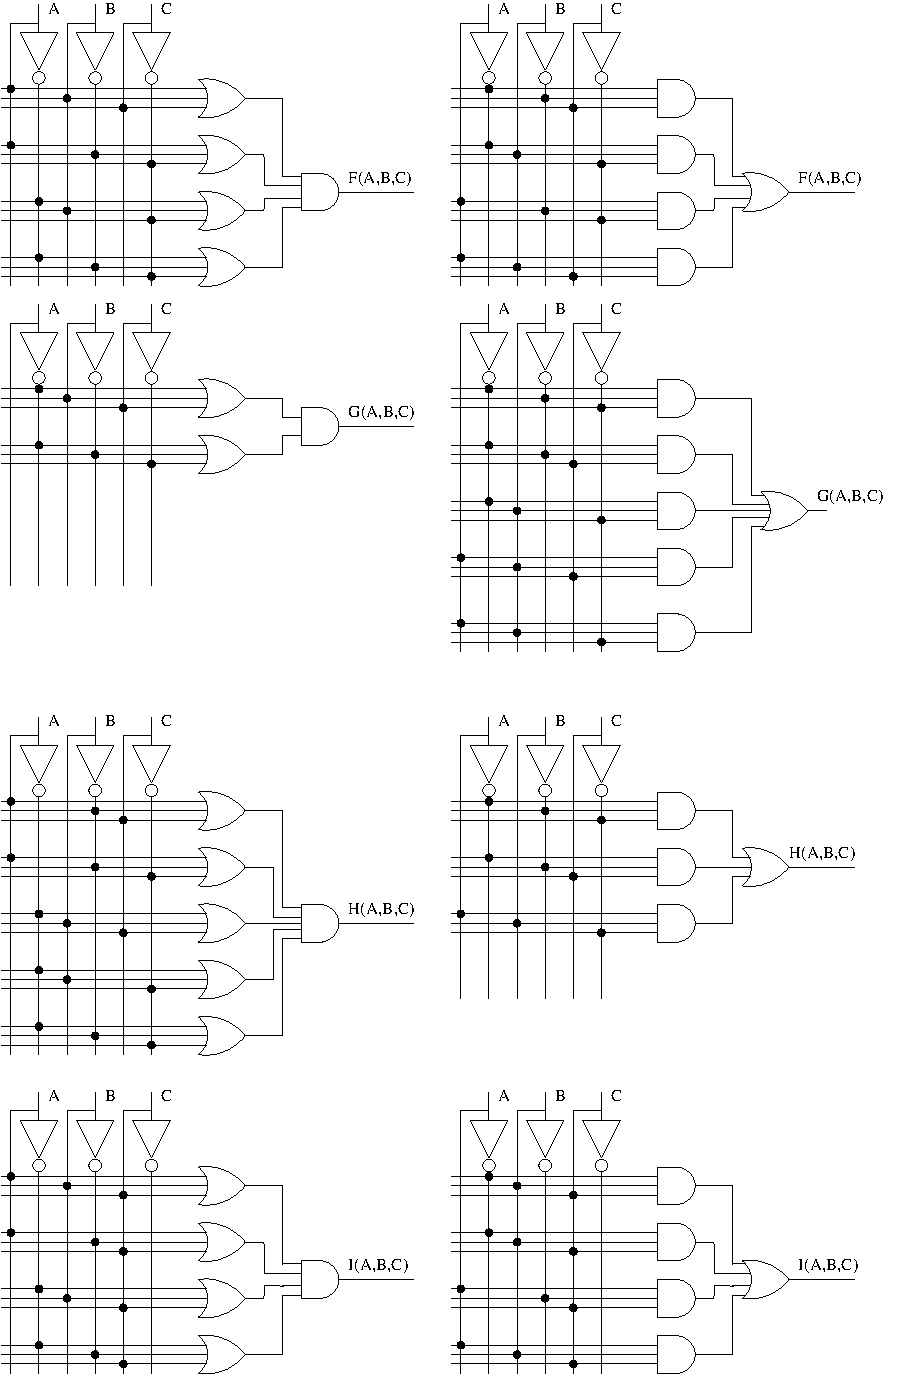
\includegraphics[max width=0.95\linewidth]{Sol2-4}
                                    \end{figure}
                                \end{onlysolution}
                        \end{enumerate}
                        Treat each output independently of the other.  For example when
                        working with function $I$, cover up the columns $F,G$ and $H$.

                        $$
                        \begin{array}{c|c|c||c|c|c|c}
                            A & B & C & F & G & H & I \\ \hline \rowcolor{gray!15}
                            0 & 0 & 0 & 0 & 1 & 1 & 0 \\ \hline
                            0 & 0 & 1 & 1 & 1 & 1 & 1 \\ \hline \rowcolor{gray!15}
                            0 & 1 & 0 & 1 & 1 & 0 & 0 \\ \hline
                            0 & 1 & 1 & 0 & 1 & 0 & 1 \\ \hline \rowcolor{gray!15}
                            1 & 0 & 0 & 1 & 0 & 0 & 0 \\ \hline
                            1 & 0 & 1 & 0 & 1 & 0 & 1 \\ \hline \rowcolor{gray!15}
                            1 & 1 & 0 & 0 & 1 & 1 & 0 \\ \hline
                            1 & 1 & 1 & 1 & 0 & 0 & 1 \\ \hline
                        \end{array}$$

                    \item  \textbf{ (2 pts. each)} Prove the validity of the following
                        statements using the laws of Boolean Algebra. For each step of
                        the proof, identify which law was used.
                        \begin{enumerate}
                            \item $X'Y' + XY + X'Y = X' + Y$

                                \begin{onlysolution}  \textbf{Solution}
                                    \begin{align*}
                                        &X'Y' + XY + X'Y =          & 3D\\
                                        &X'Y' + X'Y + XY+ X'Y =     & 8 \\
                                        &X'(Y' + Y )+ Y(X+ X')Y=    & 5 \\
                                        &X' + Y                     & \textbf{{QED}} \\
                                    \end{align*}
                                \end{onlysolution}

                            \item $(X+Y')X'Y' = X'Y'$

                                \begin{onlysolution}  \textbf{Solution}
                                    \begin{align*}
                                        &(X+Y')X'Y' =     & 8 \\
                                        &XX'Y + X'Y'Y' =  & 5D \\
                                        &0+X'Y'=          & 1 \\
                                        &X'Y'             & \textbf{{QED}} \\
                                    \end{align*}
                                \end{onlysolution}

                            \item $(X+Y)(X'+Z) = XZ + X'Y$

                                \begin{onlysolution}  \textbf{Solution}
                                    \begin{align*}
                                        &(X+Y)(X'+Z) =             & 8     \\
                                        &(X+Y)X' + (X+Y)Z =        & 8     \\
                                        &XX' + YX' + XZ + YZ =     & 1D,5  \\
                                        &YX' + XZ + YZ(X+X') =     & 8     \\
                                        &YX' + XZ + XYZ + X'YZ =   & 6     \\
                                        &X'Y + X'YZ + XZ + XYZ =   & 1D, 8 \\
                                        &X'Y(1+Z) + XZ(1+Y) =      & 2, 1D \\
                                        &X'Y + XZ                  & \textbf{{QED}}   \\
                                    \end{align*}
                                \end{onlysolution}
                                \filbreak
                            \item $X'Y' + (X+Y)Z = X'Y' + Z$

                                \begin{onlysolution}  \textbf{Solution}
                                    \begin{align*}
                                        &X'Y' + (X+Y)Z =                                & 8\\
                                        &X'Y' + XZ + YZ =                               & 1D,5 \\
                                        &X'Y'*(Z+Z') + XZ + YZ(X+X') =                  & 8 \\
                                        &X'Y'Z' + X'Y'Z + XZ + XYZ + X'YZ =             & 3 \\
                                        &X'Y'Z' + X'Y'Z + X'Y'Z + XZ + XYZ + X'YZ =     & 8 \\
                                        &X'Y'(Z+Z') + XZ(1+Y) + X'Z(Y'+Y) =             & 5,1D \\
                                        &X'Y' + XZ + X'Z  =                             & 8 \\
                                        &X'Y' + Z(X+X') =                               & 5, 1D\\
                                        &X'Y' + Z                                       & \textbf{{QED}} \\
                                    \end{align*}
                                \end{onlysolution}

                            \item $A'C+BC+AB = A'C+AB$
                                \begin{onlysolution}  \textbf{Solution}
                                    \begin{align*}
                                        &A'C + BC+AB =                          & 1D, 5 \\
                                        &A'C + (A+A')BC + AB(C+C')              & 8  \\
                                        &A'C + ABC + A'BC + ABC + ABC'=         & 3\\
                                        &A'C + A'BC + ABC + ABC'=               & 8\\
                                        &A'C(1+B) + AB(C+C')=                   & 5, 1D\\
                                        &A'C + AB                               & \textbf{{QED}} \\
                                    \end{align*}
                                \end{onlysolution}
                            \item $A(B+C)=AB+AB'C$

                                \begin{onlysolution}  \textbf{Solution}
                                    \begin{align*}
                                        &AB+AB'C=                           & 1D,5  \\
                                        &AB(C+C') + AB'C=                   & 8     \\
                                        &ABC+ABC'+AB'C=                     & 3     \\
                                        &ABC + ABC + ABC' + AB'C=           & 6     \\
                                        &ABC + ABC' + ABC + AB'C=           & 8     \\
                                        &AB(C+C'+C) + AB'C =                & 8     \\
                                        &AB + AB'C=                         & \textbf{{QED}}   \\
                                    \end{align*}
                                \end{onlysolution}

                                \filbreak
                            \item $(A+B+C)(A+B+C')(A'+B+C')(A'+B'+C') = (A+B)(A'+C')$

                                \begin{onlysolution}  \textbf{Solution}
                                    \begin{align*}
                                        &(A+B+C)(A+B+C')(A'B+C')(A'+B'+C')=             & 4\\
                                        &((A+B+C)(A+B+C')(A'B+C')(A'+B'+C'))''=         & 9D\\
                                        &(A'B'C + A'B'C' + AB'C + ABC)'=                & 8\\
                                        &(A'B'(C+C') + AC(B'+B))'=                      & 5, 1D\\
                                        &(A'B' + AC)'=                                  & 9 \\
                                        &(A+B)(A'+C')=                                  & \textbf{{QED}}  \\
                                    \end{align*}
                                \end{onlysolution}
                        \end{enumerate}

                    \item \textbf{ (4 pts.)} Design a circuit called MUX2.  MUX2 has three bits
                        of input $S, y_0, y_1$ and one bit of output $F$.  If $S=0$, then
                        $F=y_0$; else if $S=1$, then $F=y_1$.
                        \begin{enumerate}
                            \item Write down the truth table for the MUX2 function.

                                \begin{onlysolution}  \textbf{Solution} \itshape

                                    \begin{tabular}{l|l|l|l}
                                        S & $y_0$ &  $y_1$ & F  \\ \hline \rowcolor{gray!15}
                                        0 & 0  &  0  & 0        \\ \hline
                                        0 & 0  &  1  & 0        \\ \hline \rowcolor{gray!15}
                                        0 & 1  &  0  & 1        \\ \hline
                                        0 & 1  &  1  & 1        \\ \hline \rowcolor{gray!15}
                                        1 & 0  &  0  & 0        \\ \hline
                                        1 & 0  &  1  & 1        \\ \hline \rowcolor{gray!15}
                                        1 & 1  &  0  & 0        \\ \hline
                                        1 & 1  &  1  & 1        \\
                                    \end{tabular}
                                \end{onlysolution}

                            \item Determine the canonical SOP realization for MUX2;
                                do not simplify.

                                \begin{onlysolution}  \textbf{Solution}
                                    $F = S' y_0 y_1' + S' y_0 y_1 + S y_0' y_1 + S y_0 y_1$
                                \end{onlysolution}
                        \end{enumerate}

                    \item \textbf{ (6 pts.)} Design a circuit called MUX4.  MUX4 has six bits of input
                        $S_1 S_0, y_0, y_1, y_2, y_3$ and one bit of output $F$.  \\
                        If      $S_1 S_0 = 00$ then $F=y_0$  \\
                        else if $S_1 S_0 = 01$ then $F=y_1$ \\
                        else if $S_1 S_0 = 10$ then $F=y_2$ \\
                        else if $S_1 S_0 = 11$ then $F=y_3$ \\
                        Without writing down the truth table determine a SOP expression
                        to realize F by listing all possible inputs which will cause F to equal 1.
                        Then try to simplify your expression using Boolean Algebra.

                        \begin{onlysolution}  \textbf{Solution} \itshape

                            The output F only equals one in the following cases.
                            \begin{description}
                                \item S1=0 S0=0 and y0=1
                                \item S1=0 S0=1 and y1=1
                                \item S1=1 S0=0 and y2=1
                                \item S1=1 S0=1 and y3=1
                            \end{description}

                            With this information we can form four product terms, one for each input,
                            that equal 1 only for that input.  ORing together these product terms
                            will give us the solution to the problem.

                            $F = S_1'S_0'y_0 + S_1'S_0 y_1 + S_1 S_0'y_2 + S_1 S_0 y_3$
                        \end{onlysolution}

                    \item  \textbf{ (4 pts.)} Design a logic circuit called \textit{MAJ} which
                        has three inputs $A,B,C$ and one output $Z$. The output equals 1
                        when a majority of the inputs are equal to 1, otherwise the output is 0.
                        \begin{enumerate}
                            \item Write the truth table for the MAJ function.

                                \begin{onlysolution}  \textbf{Solution} \itshape

                                    \begin{tabular}{l|l|l||l}
                                        A & B & C &  F \\ \hline \rowcolor{gray!15}
                                        0 & 0 & 0 &  0 \\ \hline
                                        0 & 0 & 1 &  0 \\ \hline \rowcolor{gray!15}
                                        0 & 1 & 0 &  0 \\ \hline
                                        0 & 1 & 1 &  1 \\ \hline \rowcolor{gray!15}
                                        1 & 0 & 0 &  0 \\ \hline
                                        1 & 0 & 1 &  1 \\ \hline \rowcolor{gray!15}
                                        1 & 1 & 0 &  1 \\ \hline
                                        1 & 1 & 1 &  1 \\
                                    \end{tabular}
                                \end{onlysolution}

                            \item Determine the canonical SOP realization for the MAJ
                                function, do not simplify.

                                \begin{onlysolution}  \textbf{Solution}
                                    $F = A'BC + AB'C+ABC'+ABC$
                                \end{onlysolution}
                        \end{enumerate}

                    \item \textbf{ (4 pts.)} Let $X$ and $Y$ each be 2-bit signals whose
                        elements are $x_1 x_0$ and $y_1 y_0$ respectively.  Determine the
                        $\sum m$ and $\prod M$ expression for a circuit whose 1-bit
                        output $z$ is defined by the following statement.
\begin{verbatim}
        if (X == Y) then z = 1 else z = 0
\end{verbatim}
                        \begin{onlysolution}  \textbf{Solution} \itshape
                            $$
                            \begin{array}{c|c|c|c||c|c||c}
                                a_1 & a_0 & b_1 & b_0 & A  & B & z  \\ \hline \rowcolor{gray!15}
                                0 & 0 & 0 & 0 & 0 & 0 & 1           \\ \hline
                                0 & 0 & 0 & 1 & 0 & 1 & 0           \\ \hline \rowcolor{gray!15}
                                0 & 0 & 1 & 0 & 0 & 2 & 0           \\ \hline
                                0 & 0 & 1 & 1 & 0 & 3 & 0           \\ \hline \rowcolor{gray!15}
                                0 & 1 & 0 & 0 & 1 & 0 & 0           \\ \hline
                                0 & 1 & 0 & 1 & 1 & 1 & 1           \\ \hline \rowcolor{gray!15}
                                0 & 1 & 1 & 0 & 1 & 2 & 0           \\ \hline
                                0 & 1 & 1 & 1 & 1 & 3 & 0           \\ \hline \rowcolor{gray!15}
                                1 & 0 & 0 & 0 & 2 & 0 & 0           \\ \hline
                                1 & 0 & 0 & 1 & 2 & 1 & 0           \\ \hline \rowcolor{gray!15}
                                1 & 0 & 1 & 0 & 2 & 2 & 1           \\ \hline
                                1 & 0 & 1 & 1 & 2 & 3 & 0           \\ \hline \rowcolor{gray!15}
                                1 & 1 & 0 & 0 & 3 & 0 & 1           \\ \hline
                                1 & 1 & 0 & 1 & 3 & 1 & 0           \\ \hline \rowcolor{gray!15}
                                1 & 1 & 1 & 0 & 3 & 2 & 0           \\ \hline
                                1 & 1 & 1 & 1 & 3 & 3 & 1           \\
                            \end{array}$$

                            Yielding

                            $z = \sum m(0,5,10,15) = \prod M(1,2,3,4,6,7,8,9,11,12,13,14)$
                        \end{onlysolution}

                    \item \textbf{ (4 pts.)} Let $X$ and $Y$ each be 2-bit signals whose
                        elements are $x_1 x_0$ and $y_1 y_0$, respectively.  Determine the
                        $\sum m$ and $\prod M$ expressions for a circuit whose 1-bit
                        output $z$ is defined by the following statement.
\begin{verbatim}
        if (X + Y > 3) then z = 0 else z = 1
\end{verbatim}

                        \begin{onlysolution}  \textbf{Solution}
                            $$
                            \begin{array}{c|c|c|c||c|c||c}
                                a_1 & a_0 & b_1 & b_0 & A  & B & z  \\ \hline \rowcolor{gray!15}
                                0 & 0 & 0 & 0 & 0 & 0 & 1           \\ \hline
                                0 & 0 & 0 & 1 & 0 & 1 & 1           \\ \hline \rowcolor{gray!15}
                                0 & 0 & 1 & 0 & 0 & 2 & 1           \\ \hline
                                0 & 0 & 1 & 1 & 0 & 3 & 1           \\ \hline \rowcolor{gray!15}
                                0 & 1 & 0 & 0 & 1 & 0 & 1           \\ \hline
                                0 & 1 & 0 & 1 & 1 & 1 & 1           \\ \hline \rowcolor{gray!15}
                                0 & 1 & 1 & 0 & 1 & 2 & 1           \\ \hline
                                0 & 1 & 1 & 1 & 1 & 3 & 0           \\ \hline \rowcolor{gray!15}
                                1 & 0 & 0 & 0 & 2 & 0 & 1           \\ \hline
                                1 & 0 & 0 & 1 & 2 & 1 & 1           \\ \hline \rowcolor{gray!15}
                                1 & 0 & 1 & 0 & 2 & 2 & 0           \\ \hline
                                1 & 0 & 1 & 1 & 2 & 3 & 0           \\ \hline \rowcolor{gray!15}
                                1 & 1 & 0 & 0 & 3 & 0 & 1           \\ \hline
                                1 & 1 & 0 & 1 & 3 & 1 & 0           \\ \hline \rowcolor{gray!15}
                                1 & 1 & 1 & 0 & 3 & 2 & 0           \\ \hline
                                1 & 1 & 1 & 1 & 3 & 3 & 0           \\
                            \end{array}$$
                            Leading to the answer
                            $ z = \sum m(0,1,2,3.4,5,6,8,12) = \prod M(7,9,10,11,13,14,15)$
                        \end{onlysolution}

                    \item \textbf{ (3 pts.)} Determine the canonical SOP and POS expression for
                        $F(A,B,C) = \prod M (0,1,4,5)$  Hint, compose the truth table for $F$.

                        \begin{onlysolution}  \textbf{Solution}
                            \begin{align*}
                                F(A,B,C)&=A'BC' + A'BC +ABC' +ABC  \\
                                F(A,B,C)&=(A+B+C)(A+B+C')(A'+B+C)(A'+B+C')
                            \end{align*}
                        \end{onlysolution}

                    \item \textbf{ (3 pts.)} Determine the canonical SOP and POS expression for
                        $F(A,B,C,D) = \sum m(0,4,12,15)$ Hint, write out the truth table for $F$.

                        \begin{onlysolution}  \textbf{Solution}
                            \begin{align*}
                                F(A,B,C)=&A'B'C'D' + A'BC'D' + ABC'D' + ABCD  \\
                                F(A,B,C)=&(A+B+C+D')(A+B+C'+D)(A+B+C'+D') (A+B'+C+D') \\
                                &(A+B'+C'+D)(A+B'+C'+D')(A'+B+C+D)(A'+B+C+D')\\
                                &(A'+B+C'+D)(A'+B+C'+D')(A'+B'+C+D')(A'+B'+C'+D)
                            \end{align*}
                        \end{onlysolution}

                        \filbreak
                    \item \textbf{ (4 pts.)} For the function $F(A,B,C)= BC+AB'C'$,  draw
                        a timing diagram for an input sequence that follows the same order
                        as the rows of the truth table.  Assume a propagation delay for NOT,
                        AND and OR gate are all 10nS.
                        \begin{onlysolution}  \textbf{Solution} \itshape
                            skipped for now
                        \end{onlysolution}

                    \item \textbf{ (4 pts.)} Complete the timing diagram in Figure~\ref{fig:HWtime}
                        for the functions
                        $F(A,B,C) = AB' + BC + ABC'$ and $G(A,B,C) = (A+B')C + (BC')'$
                        \begin{figure}[ht]
                            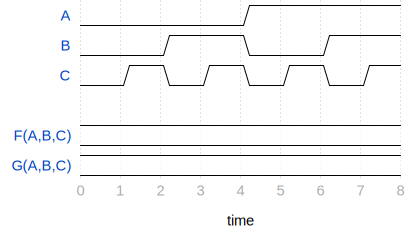
\includegraphics{wavedromFunctionToTimeProblem}
                            \caption{The timing diagram for two functions, $F(A,B,C)$ and $G(A,B,C)$.}
                            \label{fig:HWtime}
                        \end{figure}
                        \filbreak
                        \begin{onlysolution}  \textbf{Solution}
                            \begin{figure}[h!]
                                
\includegraphics{Sol2-14}
                            \end{figure}
                        \end{onlysolution}
                        \filbreak
                    \item\textbf{ (16 pts.)} Design a circuit to control
                        the water pump of a washing machine.  The pump will not pump
                        water if
                        \begin{description}
                            \item The lid is closed and the cycle is not fill
                            \item The cycle is fill and the detergent level is empty
                            \item The detergent is not empty and the lid is open
                        \end{description}

                        The variables for this problem are:
                        \begin{description}
                            \item L = lid is closed
                            \item C = cycle is fill
                            \item D = detergent is empty
                            \item P = pump will pump water
                        \end{description}

                        Create a truth table which describes when the pump will not
                        pump water.  Call this output P'.  Determine the canonical SOP
                        expression for P'.  Use this canonical SOP expression to generate
                        a circuit diagram for P.  This can be done by inserting an
                        inverter onto the output of the circuit.

                        Take the P' column from truth table and invert all the entries
                        to generate a new output column called P (because
                        the negation of P' is P).  Determine the canonical SOP
                        realization for P using this new column.

                    \item\textbf{Lab}
                        Design a hexadecimal-to-seven-segment display (hex2SevenSegment) digital circuit.
                        The hex2SevenSegment circuit
                        converts a 4-bit input that represents a hexadecimal digit to  a 7-bit output that
                        displays the hexadecimal
                        digit on a 7-segment display as shown in Figure~\ref{figure:he2SevenToDisplay}.  A
                        7-segment display is an
                        figure-8 shaped arrangement of 7 LEDs that can be individually illuminated.

                        \begin{figure}[ht]
                            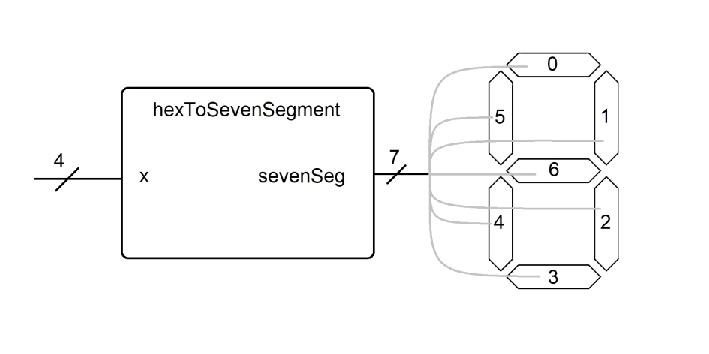
\includegraphics{hex2SevenToDisplay}
                            \caption{The connection beteen the 4-bit input nd the 7-segment display. }
                            \label{figure:he2SevenToDisplay}
                        \end{figure}

                        Each of the 7 LEDs is associated with the output from the hex2SevenSegment circuit
                        as shown in Figure~\ref{figure:dataPathControlSevenSegmentLayout}A.  Active high LEDs
                        illuminate when
                        their input is logic 1 and turn-off when their input of logic 0.  If the LEDs of a
                        7-segment display are active
                        then a binary input of 1100110 would display the pattern shown in
                        Figure~\ref{figure:dataPathControlSevenSegmentLayout}B

                        \begin{figure}[ht]
                            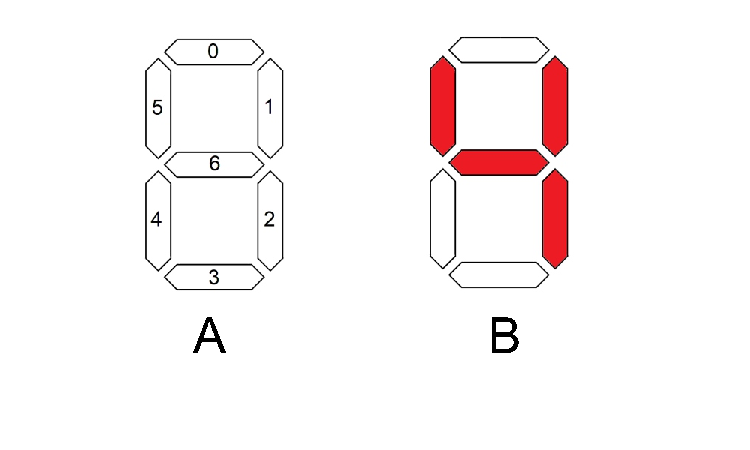
\includegraphics{sevenSegmentLayout}
                            \caption{A) The individual segments of a 7-segment display and their bit position
                            in the 7-bit
                            output from the he2SevenSegment circuit.
                    b) The illumination patter for the digit ``4'' }
                    \label{figure:dataPathControlSevenSegmentLayout}
                \end{figure}

                Since there are many different ways to illuminate the 7 segments to form the characters 0
                \ldots F, we will
                standardize our
                pattern to those shown in Figure~\ref{figure:dataPathControlSevenSegmentPatterns}.

                \begin{figure}[ht]
                    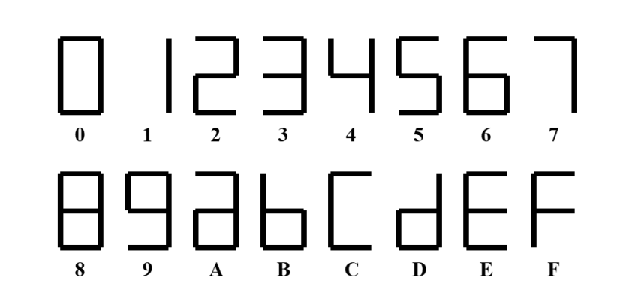
\includegraphics{sevenSegmentPatterns}
                    \caption{The illuminated patterns for all 16 inputs. }
                    \label{figure:dataPathControlSevenSegmentPatterns}
                \end{figure}

                The truth table for the hex2SevenSegment circuit is started below.  Complete the
                truth table by filling the outputs for the seg column.  Note that the number inside the
                square brackets is the bit index in the 7-bit output.  The relationship between the
                bit index and the segments is shown in Figure~\ref{figure:he2SevenToDisplay}.

                \begin{tabular}{l|l|l|l|l|l|l|l}
                    x        & seg[6] & seg[5] & seg[4] & seg[3] & seg[2] & seg[1] & seg[0]  \\ \hline
                    0000 &           &             &            &           &            &            &   \\ \hline
                    0001 &           &             &            &           &            &            &   \\ \hline
                    0010 &           &             &            &           &            &            &   \\ \hline
                    0011 &           &             &            &           &            &            &   \\ \hline
                    0100 &   1       &    1        &     0      &     0     &     1      &      1     & 0 \\ \hline
                    0101 &           &             &            &           &            &            &   \\ \hline
                    0110 &           &             &            &           &            &            &   \\ \hline
                    0111 &           &             &            &           &            &            &   \\ \hline
                    1000 &           &             &            &           &            &            &   \\ \hline
                    1001 &           &             &            &           &            &            &   \\ \hline
                    1010 &           &             &            &           &            &            &   \\ \hline
                    1011 &           &             &            &           &            &            &   \\ \hline
                    1100 &           &             &            &           &            &            &   \\ \hline
                    1101 &           &             &            &           &            &            &   \\ \hline
                    1110 &           &             &            &           &            &            &   \\ \hline
                    1111 &           &             &            &           &            &            &   \\
                \end{tabular}

                Now determine the \SOPmin expression for each of the 7 outputs.

        \end{enumerate}
